\documentclass[12pt]{article}
\usepackage[utf8]{luainputenc}
\usepackage[babel, titelside, nat, farve, da]{ku-forside}
\usepackage{cite}
\usepackage{amsfonts}
\usepackage{amsmath}
\usepackage[obeyspaces,spaces]{url}
\usepackage{hyperref}
\usepackage{graphicx}
\usepackage{caption}
\usepackage{subcaption}
\usepackage{gantt}
\usepackage[section]{placeins}

\hypersetup{pdfborder = {0 0 0}}

\opgave{Bachelorprojekt}
\forfatter{Christoffer Wadum Larsen og Lasse Ahlbech Madsen}

\titel{Substitute CT til brug ved PET rekonstruktion}
\undertitel{}

\vejleder{Sune Darkner}
\dato{16-06-2014}

\begin{document}
\maketitle
\newpage
\abstract

\textbf{Formål:} Undersøg brugbarheden af sCT til rekonstruktion af PET og vurdér kvaliteten. Undersøg desuden om sCT er stabilt over tid. \textbf{Resultat:} Flere regioner i hjernen på PET baseret på sCT har forskelle på mere end 10\% i forhold til PET baseret på CT. Værdierne på sCT billedet ser ud til at falde med tiden. \textbf{Konklusion:} Kvaliteten af sCT ser ikke ud til at være god nok til generelt brug. Det er muligt den kan bruges ved diagnosticering af Alzheimers. Værre endnu, så ser det ud til at metoden ikke er stabil. Periodiske beregninger af modeller ser derfor ud til at være nødvendige.\\

\textbf{Purpose:} Investigate the usefulness of sCT in PET reconstruction and evaluate the quality. Further investigate if the sCT is stable with time. \textbf{Result:} Several regions of the brain in the PET image based on sCT shows differences larger than 10\% difference compared to PET image based on CT. \textbf{Conclusion:} The quality of sCT seems to be too low for general use. It is possible the sCT could be used in diagnosing Alzheimer's disease. Even worse, the method proves not to be stable over time. Thus periodic calculation of the model seems to be necessary.

\newpage
\section{Forord}

Dette er vores bachelorprojekt, som vi har lavet i perioden 3.
februar til 16. juni 2014. Vi har skrevet det hos Datalogisk Institut
ved Københavns Universitet i samarbejde med Rigshospitalet. Vores
hovedvejleder har været Adjunkt Sune Darkner med ekstern vejleder PhD,
PET/MR fysiker Adam Espe Hansen.

Vi startede dette projekt med faglige kompetencer på linje med, hvad
man kan forvente af en datalogistuderende på tredje år. Det vil sige
ingen reel erfaring med billedebehandling og maskinlæring. På begge
felter har vi i løbet af projektet tilegnet os viden om metoder og
teknikker, som vi sidenhen har benyttet.

Vi har i løbet af projektet opdaget, at nogle af vores indledende
beslutninger ikke har været optimale, og nogle af dem har vi, grundet
projektets tidsramme, ikke været i stand til at udbedre.

Vi vil gerne takke PHD Flemming Andersen, Rigshospitalet, for at komme på
projektet og løbende vejledning. Vi vil gerne takke MSc Claes Ladefoged,
Rigshospitalet, for stor assistance under projektet, og flere af de
scripts vi benyttede, er lavet af ham. Tak skal det også lyde til Overlæge
Ian Law, Rigshospitalet, for at tage sig tid til at se på vores resultater
og give feedback.
Endelig skal der lyde tak til Lektor Francois Bernard Lauze, DIKU, for
hjælp med udformning af projektet og indledende vejledning.



\newpage
\tableofcontents
\newpage

\section{Introduktion}

Til diagnosticering af patienter med visse former for sygdomme i hjerneregionen, fortages der ofte scanninger vha. Positron Emission Tomography (PET). 

PET scannere fungerer ved, at man injekterer et radioaktivt sporstof
ind i et legeme. Dette sporstof flyder ud i blodet og bliver bundet
der, hvor der benyttes mest energi, for eksempel en kræftcelle i
hjernen. Dette udsender stråling, som PET scanneren kan opfange.
Strålingsaktiviteten måles for at finde ud af, hvor i legemet der er
mest aktivitet.

PET har dog visse problemer. Man fanger kun strålingskoncentration,
så det er umuligt at se knogle, luft eller blødt væv. Dette giver
problemer, da forskelligt væv afbøjer photoner i forskellige grad,
og luft næsten ikke gør, forårsager det forringelser i kvaliteten
af scanningen, da man ikke er sikker på hvad photoner har bevæget
sig igenn, og dermed, hvor meget de er blevet afbøjet. Hvis man ikke
kender dette, kan man ikke med sikkerhed bestemme deres oprindelsessted.
Dette betragtes, som den væsentligste årsag til foringelse af
billederne.\cite{vigtighedAfAttenuation} At udbedre denne forringelse er
attenuationskorrigering.

For at udbedre denne forringelse har man kombineret Computed
Tomo\-graphy- (CT) og PET scannere. CT er et røngtenstrålingsscan,
der registrerer placering af knogle. Denne information kan man bruge
til at attenuationskorrigere og dermed få et mere korrekt resultat.
CT har dog andre problemer, da den ikke indeholder information om de
bløde vævstyper i hjernen. Derudover har røntgenstråling også
en væsentligt risiko for at forårsage yderlig skade. \cite{skadeligCT}

For at registrerer det bløde væv kan Magnetic Resonance(MR) benyttes.
MR magnetiserer et legeme svagt, når dette stoppes vil legemet hurtigt
gendanne sit oprindelige magnetfelt. Hastigheden med hvilken den gendannes
afhænger af vævet. MR scanneren varierer magnetiseringen og starter og
stopper det gentagne gange for at kortlægge legemet. Dette giver billeder
af hjernevæv i høj kvalitet.

Som med CT er MR også blevet sammensat med PET til en PET/MR scanner, men
den kan ikke bruges til attenuationkorrektion, da knogle og luft begge 
gendanner deres magnetfelt så hurtigt, at det er meget svært at måle.
Effekten er at knoglen kommer til at ligne luft på billederne. Dette
problem er forsøgt løst på flere måde.

På Rigshospitalet har man hidtil kombineret MR billeder med CT
billeder for at kunne lave attenuationskorrigerede billeder kaldet FullCT.
Dette medfører dog det tidligere nævnte problem med den skadende
effekt af røngtenstråling og man skal flytte patienten rundt mellem
flere scannere. Da scanningerne er foretaget på forskellige scannere
kan man ikke forvente at patienterne ligger ens. Dette problem skal
også løses. Derfor er man særdeles interesserede i, at foretage
attenuationskorrigering alene vha. MR.

Der er to hovedretninger til at udregne CT data ud fra MR data. De
anatomiske og de voxelbaserede. De anatomiske forsøger at kortlægge
hjernen og beskrive generelle træk, de matcher patient data op imod et
udregnet atlas, og forsøger at korrigere udfra det. Det giver nogle
problemer ved atypisk anatomi, men har vist sig at producere gode
resultater~\cite{atlas1, atlas2}.

Alternativt er der voxelbaserede metoder, som for hver voxel forsøger
at bestemme hvilken type væv den tilhører, men her er det selvfølgelig
virkelig et problem, at man ikke kan skelne mellem luft og knogle.

Ved at benytte meget korte sekvenser, kaldet UTE (Ultrashort Echo Times,)
er det muligt at registrere knogle på MR-scannere. Man måler fra to
forskellige vinkler og med to forskellige echo tider. Der hvor der er
sket en markant ændring i mellem de to billeder, kan da formodes at
være knogle. Implementation af dette på Siemens scannerne, som
Rigshospitalet benytter, har dog vist sig ikke at være på højde med
kombinationen af CT og MR billeder.

Målet med denne opgave er at implementere metoden beskrevet i
Johansson et al., som kan udregne et substitut-CT (sCT) ud fra fire
UTE sekvenser og et T2-vægtet MR billede for en vilkårlig patient. Dette
vil vi gøre ved at træne en Gaussian Mixture Regression model ud fra
disse serier samt et CT målt på samme patient.


\section{Teori}
\subsection{Kort introduktion til de forskellige type data og dannelse af disse.}

\todochristoffer{Læs}
\todolasse{Skriv om PET effekt på MR. Mere om forskel på UTE-sekvenserne}


Til metoden benyttes Magnetic resonance- (MR) og Computed
tomography-billedsekvenser (CT). CT er en røngtenscanning, som måler
evnen til at blokkere stråling, hvilket har en direkte relation til
elektrondensitet. Knoglen er meget tydelig i disse billeder. MR magnetiserer
kroppen ganske svagt, når dette stoppes vil kroppens magnetisering bruge
ganske kort tid på at gendannes, og der måles på denne for at kortlægge
struktur.

Vi benytter 5 MR-sekvenser: T1, som måles efter kroppen har gendannet en vis
mændge magnetisme, og derudover 4 Ultrashort echo time MR-sekvenser (UTE)
taget fra 2 forskellige vinkler og varierende ekko tider. Når man sænker echo
tiden betydeligt bliver det muligt at se knogle på MR billeder, men ikke med
en præcision, som kan matche CT.


\subsection{Registrering}

\todochristoffer{Mangler referencer i teori til registrering}

Billeder taget på PET/MR og PET/CT skannere kan som regelt ikke processeres
sammen grundet flere faktorer. Patienten ligger sjældent præcis på samme
måde, billederne bliver taget i forskellige opløsninger og patienten kan have
implantater der forvrænger billederne og de ligger også i forskellige image
spaces. For at klargøre billederne skal de derfor co-registreres.

Ved co-registrering forsøger man at få alle billederne til at ligge i samme
rum. I forhold til MRI billederne er co-registrering ofte trivielt. At
co-registrere et MRI og CT billede er derimod vanskeligere. Derfor har vi valgt
to forskellige metoder.

\todo{Mangler der noget her?}

I samme omgang som vi co-registrere billederne er vi interesserede også
at finde en maske. Masken skal bruges til at begrænse udregningen af sCT
billedet så vi ikke bruger lang tid på at lede efter knogle i luften rundt om
patienten.

\subsection{Attenuation correction}
Ved PET billeder måles photoner fra materiale man har sprøjtet ind i blodet. Ved
at se på hvor photonerne kommer fra kan man se hvor meget blod der flyder til
forskellige steder. Det er særligt brugbart til at identificere kræftknuder i
hjernen da kræftknuderne har et højere energiforbrug, og dermed får tilført
mere blod kan man se hvor de er henne.

Normalt bruges et CT billede for at korrigere for afbøjninger, men det  

\todochristoffer{Mangler at beskrive AC}

\subsection{Artifakter i hjerner}

\todo{Mangler at beskrive artifakter}

\subsection{Statistikgøjl}

\todochristoffer{Mangler at beskrive statistikken}

\todo{Overvej ordenen på næste 3 sections}

\subsection{Arbejdsgangen}

\todochristoffer{Arbejdsgangen er ikke beskrevet}

På Rigshospitalet er fremgangsmåden med MR
hjerneskanninger, at man også laver et CT scan. T1 billedet fra MR scanneren
og CT co-registreres herefter og sammenlægges til et attenuationskorrigeret
uMap kaldet FullCT. Derudover benyttes et Dixon uMap til at sætte dimensioner
på det nye uMap. Dette rekonstrueres på hospitalets scanner.


\subsubsection{FullCT}

\todolasse{FullCT er ikke beskrevet. Snakker nærmere med Claes og justerer
også i ovenstående snit}

Det er noget funk

\subsubsection{Rekonstruktion}

\todolasse{Rekonstruktion er ikke beskrevet. Skal snakke med et par folk.
Hvordan det }


\section{Registrering}

Billeder taget på MR/PET- og PET/CT-skannere kan som regel ikke
processeres sammen grundet flere faktorer. Patienten ligger sjældent
præcis på samme måde, billederne bliver taget i forskellige
opløsninger, og de bliver optaget i forskellige billedrum. For at
klargøre billederne skal de derfor co-registreres.

Ved co-registrering forsøger man at få alle billederne til at ligge i
samme rum. I forhold til MR-billederne er co-registrering ofte trivielt.
At co-registrere et MR- og CT-billede er derimod vanskeligere. Derfor har
vi valgt to forskellige metoder.

I samme omgang, som vi co-registrerer billederne, er vi interesserede i
også at finde en maske. Masken skal bruges til at lette udregningen
af sCT-billedet, så vi ikke bruger lang tid på at lede efter knogle i
luften rundt om patienten. Masken skal også fjerne eventuel nakkestøtte og
hovedholdere på CT-billederne.

\subsection{Co-registrering af UTE- og T2-billeder}

Til co-registrering af UTE- og T2-billederne har vi valgt at bruge
Insight ToolKit (ITK)\footnote{\url{http://www.itk.org/}}. Herfra benytter vi en implementation af Mattes
Mutual Information algoritme samt lineær translation og interpolering. Vi har valgt denne implementation fordi det var foreslået i dokumentationen for ITK.

\subsection{Co-registrering af UTE- og CT-billeder}

Co-registrering af UTE- og CT-billeder er, modsat UTE/T2, en ikke-triviel
opgave. Vi har valgt en landmark baseret løsning fra MINC's toolkit\footnote{\url{http://www.bic.mni.mcgill.ca/ServicesSoftware/ServicesSoftwareMincToolK it}}.
Vi har ikke selv skrevet denne løsning, men bruger i stedet samme
løsning som Rigshospitalet.

\subsection{Generering af maske}

Til udregning af modellerne har maskerne en væsentlig betydning for korrektheden af klassifikationen. Vi har flere gange undervejs måtte ændre hvilke billeder, som vi bruger til at genskabe modellerne, og har ikke haft tid til at generere de tilhørende masker hver gang.

Hvis ikke maskerne kun dækker punkter hvor der findes data på alle 16 billeder, risikerer vi en misklassificering. 

Til generering af masken bruger vi først en implementering af Otsu
thresholding-algoritmen for at finde en binær repræsentation. For at
sikre, at vores maske ikke bliver for lille, udvider vi det binære billede
vha. en neighborhood-connected-algoritme med 2-3 pixel i x, y og z
retningerne. Til sidst inverteres billedet, hvilket efterlader os med en
binær maske.

De endelige masker vi brugte var alt for store i forhold til T2-sekvenserne, hvilket kan have haft en betydelig negativ effekt på kvaliteten af vores T2.

Da det tager forholdsvis lang tid at udregne modellerne og endnu længere tid at lave rekonstruktionerne, havde vi ikke tid til at prøve med nye masker.



\section{Metoden}
\subsection{Gaussian Mixture Model}

\subsubsection{At finde modellen}
Vi bruger en mixtur af gaussians til at beregne voxel værdier
for et sCT. For hver patient har vi 5 MR-billeder og 1 CT billede.

For at øge præcisionen udregner vi for hvert MR-billede
to nye billeder. De nye billeder beregnes ved at se på en 3x3x3
kube omkring hvert voxel og finder henholdsvis middelværdi og varians.

Herefter har vi 15 MR-billeder og 1 CT-billede som vi vil klassificere
med en mixtur af gaussians. Fra Johannson et al. ved vi at vi kan få
gode resultater med 20 gaussiske fordelinger. 

For at finde parametrene til hver gaussiske fordeling bruger vi
Expectation-Maximization (EM) algoritmen på en sammensætning af patienter
vi vil træne på. Vi starter EM algoritmen med resultatet af k-means på
dataen, hvor k er sat til 20. Dette betyder at vi ikke behøver køre
EM-algoritmen flere gang og øger sandsynligheden for et godt resultat, da
dataen allerede er klassificeret.


\todochristoffer{Matematiske ekslempler}
\todolasse{Gennemlæs}


\subsubsection{Beregning af sCT}

Vi generere sCT værdierne ved at udregne den forventede værdi af CT baseret på de 15 MR billeder. 

Som beskrevet i Johanson et al., så udregnes den forventede værdi af CT ved

\begin{equation}
(X_1 | X_2 = x_2) = \frac{\Sigma^{N}_{i=1} \bar{\mu}_{1,i} a_i h_i(x_2)}{\Sigma^{N}_{i=1} a_i h_i(x_2)}
\end{equation}

Hvor $X_1$ er CT værdien, $X_2 = (X_2 \dots X_k)$ er MR værdierne, $a_i$ er blandingsforhold og $N$ er antallet af MR billeder samt

\begin{equation}
 \bar{\mu}_{1,i} = \mu_{1,i} + \Sigma_{1 2, i} \Sigma^{-1}_{22, i}(x_2 - \mu_{2,i})
\end{equation}
og
\begin{equation}
h_i(x_2)= \frac{1}{( 2 \pi )^{k/2}|\Sigma_{22,i}|^{1/2}}\exp^{-\frac{1}{2}(x_2 - \mu_{2,i})^T \Sigma^{-1}_{22, i}(x_2 - \mu_{2,i})}
\end{equation}

$\mu_{1,i}$, $\mu_{2,i}$, $\Sigma_{1 1, i}$, $\Sigma_{1 2, i}$, $\Sigma_{2 1, i}$, $\Sigma_{2 2, i}$ er værdierne $\mu_i$ og $\Sigma_i$ estimeret med EM algoritmen og segmenteret som

\begin{equation}
\mu_i = \left(\begin{array}{c}
\mu_{i,1} \\ 1 \times 1 \\
\mu_{i,1} \\ 1 \times (k - 1)  
\end{array}\right)
\end{equation} 
\begin{equation}
\Sigma_i = \left(\begin{array}{c c}
\Sigma_{11,i} & \Sigma_{12,i} \\ 1 \times 1  & 1 \times (k-1)\\
\Sigma_{21,i} & \Sigma_{22,i} \\ (k-1) \times 1  & (k-1) \times (k-1)\\  
\end{array}\right)
\end{equation}

\todolasse{Læs}

\subsection{Hvordan han vi valgt at implementere den}

\todochristoffer{Læs}

Til metoden benytter vi for hvert træningssæt et CT, en T2 vægtet MR-sekvens
og 4 MR UTE-sekvenser. Vi benytter Insight Toolkit (ITK) til at udregne et
billede med middelværdi og et med varians for hvert MR billede.

Disse henter vi ind i matlab, hvor vi benytter fitgmdist til at lave en
gaussisk mixture fordelingsmodel. Med denne kan vi udregne et sCT udfra den
samme slags MR-sekvenser vi brugte til at lave modellen, samt deres
mean- og variansbilleder.


\section{Praktisk}

\subsection{Beregning af modellen}

Vi har valgt at implementerer metoden i Matlab da det giver os mulighed for hurtig prototyping. Derudover indeholder Matlab også en standard implementering af både k-means og EM algoritmerne.

For at beregne modellen skal vi først indlæse MR og CT billederne samt tilhørende maske for hver patient. Til det formål har vi brugt nifti_load \todo{link til toolbox}.

Herefter løber vi billederne igennem og udtager de værdier der ligger inden for masken. Alle værdier lægges i én stor 16-dimensionel liste.

For at udregne k-means bruger vi den indbyggede k-means algoritme, samt en sammensat liste med de patienter vi ønsker til grund for modellen.

Output fra k-means algoritmen gives til EM algoritmen, samt samme liste med patienter. Output herfra er vores endelige model parametre.

\todo{inkludér kode snippets}

\subsection{Beregning af sCT}

\todochristoffer{Analysen af implementeringen er ikke beskrevet}


\section{Forsøg}

Da flere af FullCT-billederne er lavet uden en perfekt maske, som skjuler hovedholder og nakkestøtten på CT-billedet, har vi valgt at generere nye FullCT, baseret på CT-billeder påført vores maske. Da støj rundt omkring hovedet påvirker attenuationkorrektionen, fik vi billeder med meget stor afvigelse imod den bagerste del af kraniet. Da vi er sikre på, at både sCT og CT billederne er påført samme maske, er der større sandsynlighed for, at vi sammenligner vores algoritme frem for støj. Der kan dog stadig fremkomme små rester af hovedstøtten tæt på kraniet, men det ser ikke ud til at være et problem.

\subsection{Validering af forsøgsresultater}

\subsubsection{Fælles histogram}

For at validere testresultaterne vil vi bl.a. benytte os af fælles histogrammer. For hvert sCT, som vi generer, har vi det korrekte CT. Ved at plotte sCT-værdier ud af y-aksen og CT værdier ud af x-aksen får vi en visuel repræsentation af ligheden mellem billederne. Hvis resultatet er identisk vil der optræde en enkelt lige linje fra $(0,0$) til $(max,max)$. Jo mere forskellige, des længere fra den lige linje ligger punkterne.

Fordelen ved denne metode er, at vi nemt kan aflæse, hvilke værdier vi har de største problemer med. Hvis vi har meget stor afvigelse i knoglerne, vil vi få en stor klump omkring 500, mens der kan være store ligheder i det bløde væv, hvilket giver en pæn linje omkring minus 500.

Derudover er det samme valideringsmetode, der bruges af Johansson et al., og vi vil derfor kunne sammenligne vores værdier med deres.

\subsubsection{Procentforskelle}

For at finde ud af om vores sCT er godt nok til attenuationskorrektion af PET-billeder, vil vi generere PET-billeder med vores sCT og det rigtige CT. Vi kan herefter konstruere et nyt billede, der er baseret på den procentvise forskel imellem FullCT-baserede PET og sCT-baserede PET. 

Ud fra procentforskelsbilledet kan vi se, hvilke regioner der er forskellige fra FullCT baserede PET-billeder, og det giver samtidigt et godt overblik over, hvor godt vores sCT-baserede PET-billede er blevet.

Begge disse valideringsmetoder er objektive, men skal evalueres manuelt. Vi forventer, at kvaliteten af sCT-billedet, og dermed også at det sCT-baserede PET-billede vil variere meget.

\subsubsection{Korrekthed}

For at bedømme korrektheden er vi nødt til at kende en parameter, som vi kan måle på. Da vi har valgt at se på procentforskelsbilleder, skal vi
derfor bestemme en procentvis afvigelse, der er godt nok til klinisk brug.
Vi har spurgt Ian Law, som er overlæge på rigshospitalet, om hvilken afvigelse
han kan acceptere, uden at det påvirker diagnosticeringen. Han mener, at
differencen i hjernen skal være under fem procent. Vi har også fundet en
artikel af Matthias Hofmann, der refererer til en grænse på ti procent~\cite{accepteretAfvigelse}. Vi
vil derfor se på billeder med en procentvis afvigelse på mindre end fem
procent som gold standard - dvs. så godt det kan blive og billeder
mellem fem og ti procent som acceptable.

\subsubsection{Regioner}

Da analyse af PET-billeder som regel er regionsbaseret, har vi valgt tre
regioner til at sammenligne. Vi har valgt lillehjernen, fordi den
typisk bliver brugt til at normalisere resten af hjernen ud fra. Derudover ved vi, at den er
et udsat område for vores modeller, da T2 ofte ikke dækker hele
lillehjernen. 

Derudover har vi valgt det forreste og det bagerste af hjernen fordi vi oplever store udslag omkring øjenhulerne og langs kanten af hjernen. Desuden er vi interesserede i, om der er den samme forskel på tværs af
hjernen, eller om den afviger mere i den ene region end den anden.

Maskerne kan ses på figur~\ref{masks}.

\begin{figure}
    \centering
   
\includegraphics[width=.5\textwidth]{billeder/masks.png}
   \caption{De tre regioner vi har målt på. Den hvide er det forreste af hovedet. Den røde er den bagerste del af hovedet, den går ikke helt ud til siderne af hovedet. Den grønne er lillehjernen.}
   \label{masks}
\end{figure}

\subsection{Leave-one-out cross validation}
\subsubsection{Fremgangsmåde}

Leave-one-out cross validation (LOOCV) er en gængs metode, der bruges til
at teste korrektheden af en algoritme. I alt sin enkelthed går metoden
ud på, at vi udvælger fem patienter. Fra de fem patienter lægger vi en
patient til side, fx. den første patient, og træner algoritmen på de
resterende fire patienter. Derefter udregner vi et sCT for den første
patient. Vi gør herefter det samme igen, men udelader patient nummer to,
træner på de resterende fire og udregner nummer to's sCT.  Ved at
rotere træningssættet får vi testet metoden med data fra forskellige
patienter, og vi får en basis for at sammenligne sCT'et.

Vi har valgt dette testscenarie for at kunne sammenligne vores resultater med Johansson et al, da de benytter samme test.

\subsubsection{Forventning}
Vi forventer at vores fælles histogrammer bliver dårligere end Johansson et al.'s, da vores hidtidige sCT er visuelt dårligere end deres.


\subsubsection{Faldgrupper}
For at opnå stabile resultater er vi nødt til at filtrere patienter med artefakter fra. Da artefakter repræsenterer områder med manglende data, tror vi, at det er nødvendigt for kvaliteten af vores algoritme, at de bliver sorteret fra.

\subsubsection{Resultat}

Eftersom det primære mål med denne test er at sammenligne os med Johansson et al., har vi valgt at lave de samme figurer.

På fælleshistogrammet i figur~\ref{fig:loocv_j_h} kan vi se to koncentrationer af punkter lige omkring 0 HU. Under nul kommer vi ud i luft og blødt væv. Over 0 kan vi se, hvordan knoglen ligger. Omkring 500 findes den største spredning af punkterne.

På det kumulative diagram på figur~\ref{fig:cumm_diff_loocv} kan vi se, at vi generelt har et problem med for lave værdier i sCT i forhold til CT. Mere end 40\% af punkterne ligger for lavt.

Ud fra procentdifference (PD) billederne på figur~\ref{col:loocv_ct}  kan vi se, at algoritmen leverer nogenlunde stabile resultater. Men vi kan også se, at der er store problemer ved ventriklerne, hvor den procentvise forskel på flere af billederne sniger sig op over de ti procent.

Hvis vi ser på et PD-billede lagt over et MR-billede, er det tydeligt, at jo tættere på kraniet man ser, des større bliver afvigelsen.

Det er ikke muligt for os at evaluere korrektheden af algoritmen omkring mund- og næseregionen, da langt de fleste T2-sekvenser ikke indeholder data så langt nede. Ligeså er der problemer i toppen af kraniet, da T2-sekvenserne også mangler en skive eller to, og derfor ikke har hele hjerneskallen med.

\begin{figure}
    \centering
    \begin{subfigure}[b]{0.47\textwidth}
    	\caption{Fælleshistogram for patient 1.}
        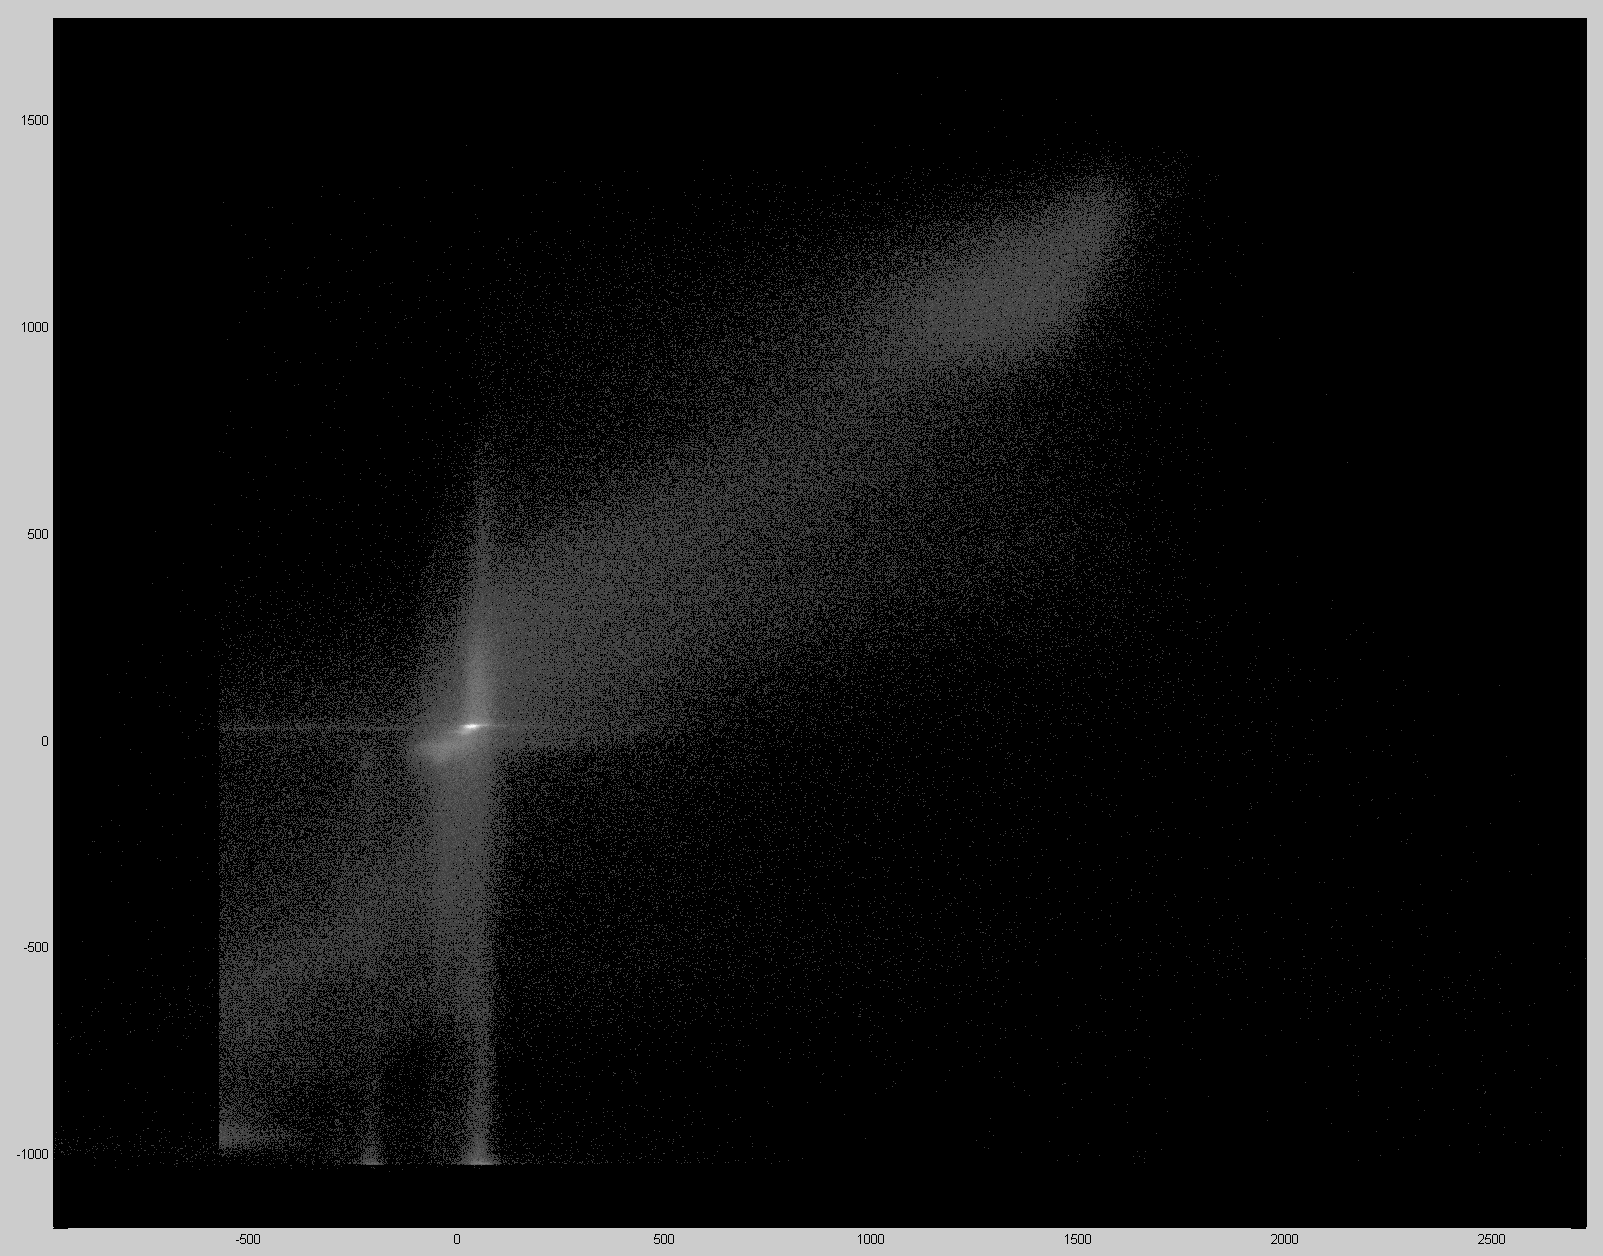
\includegraphics[width=1\textwidth]{billeder/loocv_joint_histogram.png}
        \label{fig:loocv_j_h}
    \end{subfigure}\hfill
    \begin{subfigure}[b]{0.47\textwidth}
        \caption{Kommulativt differens diagram for alle patienter i LOOCV forsøget.}
        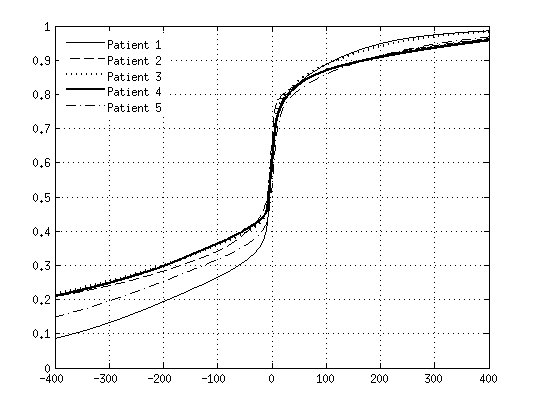
\includegraphics[width=1\textwidth]{billeder/cumm_diff_loocv.png}
        \label{fig:cumm_diff_loocv}
    \end{subfigure}
    \caption{På figur~\ref{fig:loocv_j_h} ses et fælleshistogram for patient 1. CT værdier er plottet ud af x-aksen og sCT værdier er plottet ud af y aksen. På figur~\ref{fig:cumm_diff_loocv} ses den kommulative afvigelse af sCT fra CT normaliseret til 1.}
    \label{fig:loocv}
\end{figure}

I gennemsnit er der lidt under ti procent afvigelse i selve hjernen.

\begin{figure}
    \centering
    \begin{subfigure}{0.3\textwidth}
        \centering
        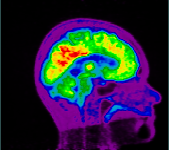
\includegraphics[width=0.75\textwidth]{colager/loocv_pet/loocv_010476_pet_ct.png}
        \caption{FullCT for patient 1.}
        \label{col:loocv_pet_pat1_ct}
    \end{subfigure}\hfill
    \begin{subfigure}{0.3\textwidth}
        \centering
        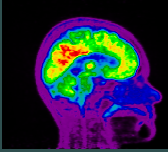
\includegraphics[width=0.75\textwidth]{colager/loocv_pet/loocv_010476_pet_sct.png}
        \caption{PET baseret på sCT.}
        \label{col:loocv_pet_pat1_sct}
    \end{subfigure}\hfill
    \begin{subfigure}{0.3\textwidth}
        \centering
        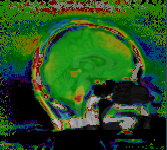
\includegraphics[width=0.75\textwidth]{colager/loocv_pet/loocv_010476_pet_pd.png}
        \caption{Procentdifferens.}
        \label{col:loocv_pet_pat1_pd}
    \end{subfigure}\\
    \begin{subfigure}{0.3\textwidth}
        \centering
        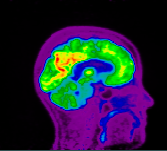
\includegraphics[width=0.75\textwidth]{colager/loocv_pet/loocv_010769_pet_ct.png}
        \caption{FullCT for patient 2.}
        \label{col:loocv_pet_pat2_ct}
    \end{subfigure}\hfill
    \begin{subfigure}{0.3\textwidth}
        \centering
        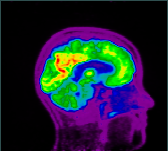
\includegraphics[width=0.75\textwidth]{colager/loocv_pet/loocv_010769_pet_sct.png}
        \caption{PET baseret på sCT.}
        \label{col:loocv_pet_pat2_sct}
    \end{subfigure}\hfill
    \begin{subfigure}{0.3\textwidth}
        \centering
        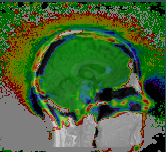
\includegraphics[width=0.75\textwidth]{colager/loocv_pet/loocv_010769_pet_pd.png}
        \caption{Procentdifferens.}
        \label{col:loocv_pet_pat2_sub}
    \end{subfigure}\\
    \begin{subfigure}{0.3\textwidth}
        \centering
        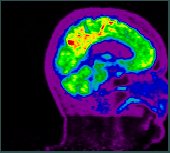
\includegraphics[width=0.75\textwidth]{colager/loocv_pet/loocv_010850_pet_ct.png}
        \caption{FullCT for patient 3.}
        \label{col:loocv_pet_pat3_ct}
    \end{subfigure}\hfill
    \begin{subfigure}{0.3\textwidth}
        \centering
        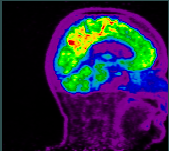
\includegraphics[width=0.75\textwidth]{colager/loocv_pet/loocv_010850_pet_sct.png}
        \caption{PET baseret på sCT.}
        \label{col:loocv_pet_pat3_sct}
    \end{subfigure}\hfill
    \begin{subfigure}{0.3\textwidth}
        \centering
        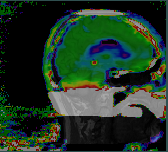
\includegraphics[width=0.75\textwidth]{colager/loocv_pet/loocv_010850_pet_pd.png}
        \caption{Procentdifferens.}
        \label{col:loocv_pet_pat3_pd}
    \end{subfigure}\\
    \begin{subfigure}{0.3\textwidth}
        \centering
        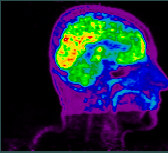
\includegraphics[width=0.75\textwidth]{colager/loocv_pet/loocv_010960_pet_ct.png}
        \caption{FullCT for patient 4.}
        \label{col:loocv_pet_pat4_ct}
    \end{subfigure}\hfill
    \begin{subfigure}{0.3\textwidth}
        \centering
        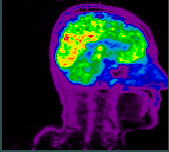
\includegraphics[width=0.75\textwidth]{colager/loocv_pet/loocv_010960_pet_sct.png}
        \caption{PET baseret på sCT.}
        \label{col:loocv_pet_pat4_sct}
    \end{subfigure}\hfill
    \begin{subfigure}{0.3\textwidth}
        \centering
        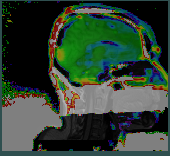
\includegraphics[width=0.75\textwidth]{colager/loocv_pet/loocv_010960_pet_pd.png}
        \caption{Procentdifferens.}
        \label{col:loocv_pet_pat4_pd}
    \end{subfigure}\\
    \begin{subfigure}{0.3\textwidth}
        \centering
        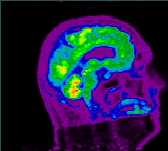
\includegraphics[width=0.75\textwidth]{colager/loocv_pet/loocv_011030_pet_ct.png}
        \caption{FullCT for patient 5.}
        \label{col:loocv_pet_pat5_ct}
    \end{subfigure}\hfill
    \begin{subfigure}{0.3\textwidth}
        \centering
        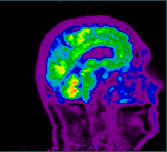
\includegraphics[width=0.75\textwidth]{colager/loocv_pet/loocv_011030_pet_sct.png}
        \caption{PET baseret på sCT.}
        \label{col:loocv_pet_pat5_sct}
    \end{subfigure}\hfill
    \begin{subfigure}{0.3\textwidth}
        \centering
        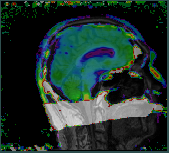
\includegraphics[width=0.75\textwidth]{colager/loocv_pet/loocv_011030_pet_pd.png}
        \caption{Procentdifferens.}
        \label{col:loocv_pet_pat5_pd}
    \end{subfigure}
    \caption{CT, sCT og procentdifferencen for de fem patienter. Farveskalaen for procentdifferencen går fra -20 til 20. Procentdifferensbilledet er også fusioneret med T1 billedet for at man kan se hvad der er hvad.}
    \label{col:loocv_pet}
\end{figure}

På FullCT-PET-rekonstruktionerne og sCT-PET-rekonstruktionerne er der
forskelle, som øjeblikkeligt falder i øjnene. I det øverste af kraniet
går der en lodret streg med luft. Den markerer, hvor T2'en stopper,
og ligeledes går der en streg gennem bunden af lillehjernen. Udenfor
hjernen ses også forskelle i næseregionen. Ved nærmere iagttagelse ses
der også andre forskelle, for eksempel er lillehjernen mere udtalt på
FullCT'en end på sCT. Udover dette virker de meget ens.

På forskelsbillederne ses ligeledes en stor forskel i top og bund af
kraniet. Derudover ses en stor forskel i ventriklerne i midten af
hjernen, men rundt om ventriklen ser forskellen ikke ud til at være så
stor. Procentforskellen i hjernen virker til at blive større tættere
på knoglen.


\begin{figure}
    \centering
    \begin{tabular}{| l | c | c | c | c |}
        \hline
         & Gennemsnit & Median & Andel over 5 \% & Andel over 10 \% \\ \hline
        Patient 1 & 6,31 \% & 4,91 \% & 48,86 \% & 13,19 \% \\ \hline
        Patient 2 & 3,38 \% & 1,67 \% & 18,33 \% & 8,16 \% \\ \hline
        Patient 3 & 3,64 \% & 2,15 \% & 19,92 \% & 18,15 \% \\ \hline
        Patient 4 & 4,15 \% & 3,35 \% & 23,76 \% & 5,16 \% \\ \hline
        Patient 5 & 2,66 \% & 1,89 \% & 10,33 \% & 3,36 \% \\ \hline
    \end{tabular}
    \caption{Tabel for forskellen i det forreste af hjernen. Læg mærke til at andelen over 10\% for alle ligger meget højt. 10\% er øverste grænse for, hvad vi kan være tilfredse med, hvilket betyder at sCT har store problemer i det forreste af hjernen.}
    \label{tab:loocv_forresthjerne}
\end{figure}

\begin{figure}
    \centering
    \begin{tabular}{| l | c | c | c | c |}
        \hline
         & Gennemsnit & Median & Andel over 5 \% & Andel over 10 \% \\ \hline
        Patient 1 & 3,99 \% & 3,73 \% & 14,98 \% & 1,1 \% \\ \hline
        Patient 2 & 1,98 \% & 1,17 \% & 6,99 \% & 3,04 \% \\ \hline
        Patient 3 & 2,28 \% & 1,28 \% & 9,42 \% & 2,89 \% \\ \hline
        Patient 4 & 4,05 \% & 3,89 \% & 17,34 \% & 1,22 \% \\ \hline
        Patient 5 & 1,84 \% & 1,45 \% & 4,11 \% & 0,65 \% \\ \hline
    \end{tabular}
    \caption{Tabel for forskellen i det bagerste af hjernen. Den bagerste del af hjernen er langt bedre end den forreste, som set på figur~\ref{tab:loocv_forresthjerne}. Det skulle egentligt være godt, men det tyder også på, at vi har store regionale problemer med sCT, hvilket er værre, end hvis hele hjernen havde været ensformigt 10\% forkert.}
    \label{tab:loocv_bagersthjerne}
\end{figure}

\begin{figure}
    \centering
    \begin{tabular}{| l | c | c | c | c |}
        \hline
         & Gennemsnit & Median & Andel over 5 \% & Andel over 10 \% \\ \hline
        Patient 1 & 4,12 \% & 2,99 \% & 18,80 \% & 5,09 \% \\ \hline
        Patient 2 & 3,74 \% & 1,94 \% & 16,84 \% & 7,00 \% \\ \hline
        Patient 3 & 7,53 \% & 5,45 \% & 53,00 \% & 24,55 \% \\ \hline
        Patient 4 & 6,45 \% & 3,06 \% & 29,86 \% & 14,29 \% \\ \hline
        Patient 5 & 11,86 \% & 5,11 \% & 50.34 \% & 34,10 \% \\ \hline
    \end{tabular}
    \caption{Tabel for forskellen i lillehjernen. Lillehjernen fortæller meget den samme historie som figur~\ref{tab:loocv_forresthjerne}. Der er dog stor usikkerhed omkring kvaliteten af sCT specielt omkring lillehjernen. Problemet stammer fra for korte T2-sekvenser.}
    \label{tab:loocv_lillehjerne}
\end{figure}


Lillehjernen er meget ustabil. Dette skyldes formentlig, at T2-sekvensen
ofte er stoppet før, den har fået nok hjerne og knogle med. Imens er der
mindre udsving forrest i hjernen, men der er stadig en stor andel, som
ligger over de 5 \%, og en del over 10 \%. Det bagerste af hjernen er
til gengæld rigtig godt, men det er en stor region, og andelen, som ligger
nær ved knoglen, er forholdsvist lav.

Generelt ligner det ikke, at der er en stabil forskel i de forskellige
regioner i de rekonstruerede hjerner, men i alle tilfælde, ud over to
tilfælde ved lillehjernen, afviger mindst halvdelen af alle voxels med
mindre end 5 \%.


\subsection{Over tid}
\subsubsection{Fremgangsmåde}

Der har fra Rigshopitalets side været en interesse i at undersøge, om
metoden ville virke fremadrettet. Altså om en model trænet på noget data
fra én periode, ville kunne bruges til at udregne et sCT for en patient
fra en helt anden periode. 

For at undersøge dette, har vi taget de seks
tidligst optagede patienter med målte UTE-sekvenser, som ikke havde artefakter, der
var nye nok til, at den T2-serie, som vi træner udfra, er optaget.
Derudover tog vi de seks nyeste UTE-patienter, ligeledes uden artefakter.

Derefter trænede vi to modeller. En på de gamle patienter og en på de
nye. Vi lavede da sCT'er for de gamle patienter på den nye model og
omvendt. For at vurdere om det virker, vil vi undersøge sammenhængen mellem værdierne i billederne, hvis de er forskellige på en ujævn måde, vil det være et problem. Det vil betyde, at man løbende skal træne nye modeller for at få gode resultater.

\subsubsection{Forventning}

Forventningen er, at de to sCT er af samme kvalitet.
Ændringer på PET/MR-scanneren kan sagtens påvirke resultaterne af et MR-scan, men så længe ændringerne er nogenlunde lige fordelt, er det ikke
et problem, da MR-units er arbitrære, og ikke kan sammenlignes fra scan til
scan. Der skal være en region af hjernen, som bliver målt anderledes i
forhold til resten af hjernen, før der bliver problemer.

\subsubsection{Faldgrupper}

Vores skanninger forløber ikke over så lang en periode, og vi har
kun valgt at sammenligne to perioder. Så det kan for det første
bare ikke have haft nogen effekt med de hidtidige ændringer, eller
måske har der været flere ændringer indimellem, som har påvirket
skanningsresultaterne, men på seneste tidspunkt er resultaterne meget
lig de tidlige.

\subsubsection{Resultat}

\begin{figure}
    \centering
    \begin{subfigure}{0.3\textwidth}
        \centering
        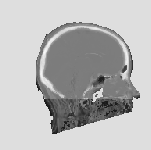
\includegraphics[width=0.75\textwidth]{colager/over_tid_sct/over_tid_sct_121280_early.png}
        \caption{Tidligt for patient 1.}
        \label{col:over_time_sct_pat1_early}
    \end{subfigure}\hfill
    \begin{subfigure}{0.3\textwidth}
        \centering
        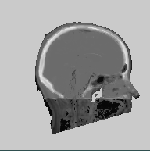
\includegraphics[width=0.75\textwidth]{colager/over_tid_sct/over_tid_sct_121280_late.png}
        \caption{Sent.}
        \label{col:over_time_sct_pat1_late}
    \end{subfigure}\hfill
    \begin{subfigure}{0.3\textwidth}
        \centering
        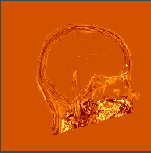
\includegraphics[width=0.75\textwidth]{colager/over_tid_sct/over_tid_sct_121280_sub.png}
        \caption{Differens.}
        \label{col:over_time_sct_pat1_sub}
    \end{subfigure}\\
    \begin{subfigure}{0.3\textwidth}
        \centering
        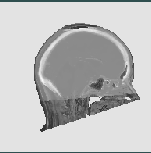
\includegraphics[width=0.75\textwidth]{colager/over_tid_sct/over_tid_sct_140547_early.png}
        \caption{Tidligt for patient 2.}
        \label{col:over_time_sct_pat2_early}
    \end{subfigure}\hfill
    \begin{subfigure}{0.3\textwidth}
        \centering
        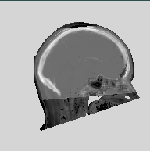
\includegraphics[width=0.75\textwidth]{colager/over_tid_sct/over_tid_sct_140547_late.png}
        \caption{Sent.}
        \label{col:over_time_sct_pat2_late}
    \end{subfigure}\hfill
    \begin{subfigure}{0.3\textwidth}
        \centering
        
\includegraphics[width=0.75\textwidth]{colager/over_tid_sct/over_tid_sct_140547_sub.png}
        \caption{Differens.}
        \label{col:over_time_sct_pat2_sub}
    \end{subfigure}\\
    \begin{subfigure}{0.3\textwidth}
        \centering
        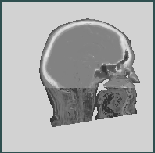
\includegraphics[width=0.75\textwidth]{colager/over_tid_sct/over_tid_sct_210445_early.png}
        \caption{Tidligt for patient 3.}
        \label{col:over_time_sct_pat3_early}
    \end{subfigure}\hfill
    \begin{subfigure}{0.3\textwidth}
        \centering
        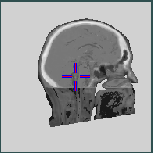
\includegraphics[width=0.75\textwidth]{colager/over_tid_sct/over_tid_sct_210445_late.png}
        \caption{Sent.}
        \label{col:over_time_sct_pat3_late}
    \end{subfigure}\hfill
    \begin{subfigure}{0.3\textwidth}
        \centering
        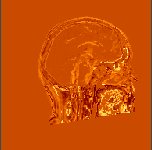
\includegraphics[width=0.75\textwidth]{colager/over_tid_sct/over_tid_sct_210445_sub.png}
        \caption{Differens.}
        \label{col:over_time_sct_pat3_sub}
    \end{subfigure}
    \caption{CT og sCT for de tre patienter. På differensbilledet er det orange ingen afvigelse. Mørkere farver går mod negativ afvigelse og lysere farver går mod positiv afvigelse.}
    \label{col:over_time_sct}
\end{figure}

\begin{figure}
    \centering
    \begin{subfigure}{0.3\textwidth}
        \centering
        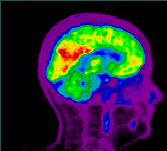
\includegraphics[width=0.75\textwidth]{colager/over_tid_pet/over_tid_121280_early.png}
        \caption{Tidligt for patient 1.}
        \label{col:over_time_pet_pat1_early}
    \end{subfigure}\hfill
    \begin{subfigure}{0.3\textwidth}
        \centering
        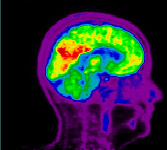
\includegraphics[width=0.75\textwidth]{colager/over_tid_pet/over_tid_121280_late.png}
        \caption{Sent.}
        \label{col:over_time_pet_pat1_late}
    \end{subfigure}\hfill
    \begin{subfigure}{0.3\textwidth}
        \centering
        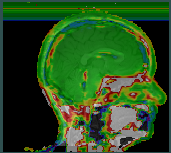
\includegraphics[width=0.75\textwidth]{colager/over_tid_pet/over_tid_121280_pd.png}
        \caption{Procentdifferens.}
        \label{col:over_time_pet_pat1_pd}
    \end{subfigure}\\
    \begin{subfigure}{0.3\textwidth}
        \centering
        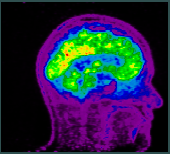
\includegraphics[width=0.75\textwidth]{colager/over_tid_pet/over_tid_140547_early.png}
        \caption{Tidligt for patient 2.}
        \label{col:over_time_pet_pat2_early}
    \end{subfigure}\hfill
    \begin{subfigure}{0.3\textwidth}
        \centering
        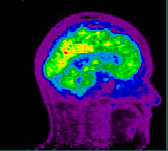
\includegraphics[width=0.75\textwidth]{colager/over_tid_pet/over_tid_140547_late.png}
        \caption{Sent.}
        \label{col:over_time_pet_pat2_late}
    \end{subfigure}\hfill
    \begin{subfigure}{0.3\textwidth}
        \centering
        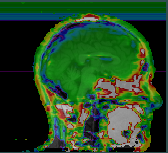
\includegraphics[width=0.75\textwidth]{colager/over_tid_pet/over_tid_140547_pd.png}
        \caption{Procentdifferens.}
        \label{col:over_time_pet_pat2_pd}
    \end{subfigure}\\
    \begin{subfigure}{0.3\textwidth}
        \centering
        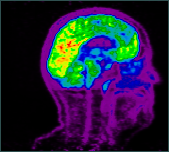
\includegraphics[width=0.75\textwidth]{colager/over_tid_pet/over_tid_210445_early.png}
        \caption{Tidligt for patient 3.}
        \label{col:over_time_pet_pat3_early}
    \end{subfigure}\hfill
    \begin{subfigure}{0.3\textwidth}
        \centering
        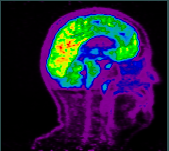
\includegraphics[width=0.75\textwidth]{colager/over_tid_pet/over_tid_210445_late.png}
        \caption{Sent.}
        \label{col:over_time_pet_pat3_late}
    \end{subfigure}\hfill
    \begin{subfigure}{0.3\textwidth}
        \centering
        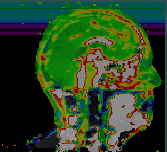
\includegraphics[width=0.75\textwidth]{colager/over_tid_pet/over_tid_210445_pd.png}
        \caption{Procentdifferens.}
        \label{col:over_time_pet_pat3_pd}
    \end{subfigure}
    \caption{Tre patienter fra midten af vores tidsperiode, hvor vi har genereret sCT ud fra modellen fra de tidlige og de sene patienter. Farveskalaen for procentdifferencen går fra -20 til 20. Procentdifferensbilledet er også fusioneret med T1-billedet, for at man kan se, hvad der er hvad.}
    \label{col:over_time_pet}
\end{figure}



På forskelsbillederne i~\ref{col:over_time_pet} er der en jævn grøn farve.
Dette tyder på en nogenlunde lige afvigelse. Der ses fejl langt kanterne
i især figur~\ref{col:over_time_pet_pat3_pd}, hvor man på de to
PET-billeder også kan se, at lillehjernen er blevet mindre på
figur~\ref{col:over_time_pet_pat3_late} end
på~\ref{col:over_time_pet_pat3_early}. Dette må formodes at være
årsagen til de store forskelle i det område. Udover dette ser det forreste af
hjernen meget ens ud, og det bagerste ligeså.

\begin{figure}
    \centering
    \begin{tabular}{| l | c | c | c | c |}
        \hline
         & Gennemsnit & Median & Andel over 5 \% & Andel over 10 \% \\ \hline
        Patient 1 & 2,28 \% & 1,49 \% & 10,06 \% & 2,27 \% \\ \hline
        Patient 2 & 2,10 \% & 1,12 \% & 9,47 \% & 2,75 \% \\ \hline
        Patient 3 & 4,54 \% & 3,78 \% & 35,15 \% & 6,26 \% \\ \hline
    \end{tabular}
    \caption{Tabel over forskellen i det forreste af hjernen mellem PET-baseret på det tidlige sCT og det sene sCT. Patient 1 og patient 2 ser begge nogenlunde ud. Desværre har patient 3 store problemer med mere end en tredjedel af værdier der er mere end 5\% forskellige.}
    \label{tab:over_tid_forresthjerne}
\end{figure}

\begin{figure}
    \centering
    \begin{tabular}{| l | c | c | c | c |}
        \hline
         & Gennemsnit & Median & Andel over 5 \% & Andel over 10 \% \\ \hline
        Patient 1 & 1,14 \% & 0,83 \% & 1,71 \% & 0,06 \% \\ \hline
        Patient 2 & 1,57 \% & 1,15 \% & 4,23 \% & 0,50 \% \\ \hline
        Patient 3 & 2,20 \% & 1,73 \% & 6,92 \% & 1,21 \% \\ \hline
    \end{tabular}
    \caption{Tabel for forskellen i det bagerste af hjernen imellem PET baseret på det tidlige sCT og det sene sCT. Her er værdierne stort set til gold standard.}
    \label{tab:over_tid_bagersthjerne}
\end{figure}

\begin{figure}
    \centering
    \begin{tabular}{| l | c | c | c | c |}
        \hline
         & Gennemsnit & Median & Andel over 5 \% & Andel over 10 \% \\ \hline
        Patient 1 & 3,00 \% & 2,70 \% & 8,14 \% & 0,62 \% \\ \hline
        Patient 2 & 2,09 \% & 1,87 \% & 3,57 \% & 0,39 \% \\ \hline
        Patient 3 & 5,71 \% & 4,50 \% & 42,45 \% & 10,20 \% \\ \hline
    \end{tabular}
    \caption{Tabel for forskellen i lillehjernen imellem PET baseret på det tidlige sCT og det sene sCT. Egentlig ser værdierne ret gode ud her. Patient 1 og 2 ligger rigtigt godt, men patient 3 har store problemer. På figur~\ref{col:over_time_pet_pat3_pd} kan vi se T2-sekvensen ikke er gået langt nok ned, derfor kan vi ikke stole på værdierne for patient 3.}
    \label{tab:over_tid_lillehjerne}
\end{figure}

Patient 1 og 2 (~\ref{tab:over_tid_lillehjerne},
~\ref{tab:over_tid_lillehjerne} og ~\ref{tab:over_tid_lillehjerne})
varierer meget lidt på tværs af de to modeller. De højere forskelle
ligger tæt ved knoglen, og selv i de områder forbliver forskellen for
det meste under de 10 \%. Patient 3 har meget høje forskelle både forrest
i hjernen og i lillehjernen. 


\section{Diskussion}

\subsection{Kvalitet af sCT}


Vi har genereret en del flere sCT som ikke er blevet brugt i rekonstruktioner,  og de fleste er blevet af ret god kvalitet, som kan ses på figur~\ref{loocv_ct}. Omkring 20\% af sCT billederne har dog større problemer i selve hjernen.

\begin{figure}
   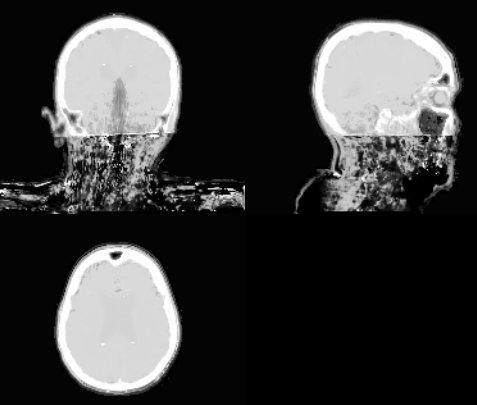
\includegraphics[width=\textwidth]{billeder/sct_problemer.png}
   \caption{sCT med problemer i hjernen. Der er mange punkter med både meget lave og meget høje værdier spredt rundt i selve hjernen.}
   \label{sct_problemer}
\end{figure}

På figur~\ref{sct_problemer} kan man se mange steder med lave værdier mellem knoglen og hjernen. Også inde i midten af hjernen er der problemer med både for høje og lave værdier. Vi er ikke klar over hvorfor nogen patienter bliver meget dårligere end de fleste andre, men Johansson et al. nævner at der kan være problemer med sampling mønstret for UTE sekvenserne.

Det er tydeligt at se ventriklerne på de fleste sCT billeder, hvilket man ikke kan på CT billederne i samme grad.

Et væsentligt problem for sCT billederne ligger i at knoglerne bliver tykkere end på de rigtige CT billeder. Til gengæld ligger værdierne for sCT knoglerne i gennemsnit under værdierne i CT knoglerne, så vi ved ikke om det har en stor eller lille indflydelse på PET rekonstruktionen.

\subsection{Sammenligning med Johansson et al}


Som det ses på figur~\ref{fig:cumm_diff_loocv} er de fleste af vores sCT dårligere kvalitet i forhold til Johansson et al. Patient 1 følger nogenlunde samme kurve som Johansson et al. har fundet frem til. Ligeledes, hvis vi ser på figur~\ref{fig:loocv_j_h}, får vi samme features som Johansson et al. fremhæver.


Vi er ikke sikre på hvorfor vores de fleste af vores sCT er blevet dårligere. Vi tror det er en kombination af flere ting. 


For det første er vores masker ikke optimale, hvilket kan resultere i dårlige modeller. For det andet kan registreringen af sCT og CT ligge en smule forkert. Eftersom vi sammenligner på voxel niveau kræver det at registreringen er så tæt på perfekt som muligt, hvis alt er forskudt bare en enkelt voxel kan det gøre en stor forskel. For det tredje har de formentligt brugt patienter med bedre T2 billeder.


Dog mener vi ikke det har noget med algoritmen at gøre. Vi bruger EM, initialiseret med k-means, hvilket gerne skulle give det samme output hver gang. Da Johansson et al. bruger samme fremgangsmetode mener vi derfor problemet ligger i forbehandlingen af billederne.


Vi prøvede at træne med dobbelt så mange patienter, for at se om det gav bedre resultater, men det havde ikke nogen mærkbar effekt på sCT billederne.


\subsection{Billedformater}

I løbet af projektet har vi oplevet en del problemer med konverteringer
mellem filtyper. Vi benyttertre forskellige. Siemens scannerne producerer
Dicom billeder som vi arbejder med i Osirix, der er et medicinsk
billedbehandlisk program. Men det er et meget stort format, der ikke er
let at arbejde med. 

På Rigshospitalet er normen at konvertere til Minc, men vi havde planer,
om at bruge ITK, og Nifti var bedre understøttet i det. I sidste ende
endte vi med at registrere vores CT billeder i Minc, så vores billeder gik
igennem alle tre typer. 

Fra Dicom til Minc mister man en skalar, som man skal tage højde for, når
man konvertere tilbage. Ved konvertering fra Minc til Nifti, hvilket vi
kun gør med vores registrerede CT billeder, bliver de laveste værdier til
-1024, dem trækker vi endnu 1025 fra, så de kommer til at matche vores
laveste værdier.

\todo{Uddyb tab ved Dicom til Minc}

At konvertere til Dicom er ikke helt trivielt, så vi konverterer først til
Minc, hvor vi lægger 2048 til for at gøre op for det offset, der skete ved
den tidligere konvertering. 

Mange af disse problemer har vi opdaget så sent i processen, at vi ikke
har kunnet nå at tage hånd om dem. Den gennemsnitlige værdi i alle vores
Nifti billeder, som vi har trænet og testet på, har været for lav, og at
lægge en værdi til ved tilbagekonverteringen udbedrer det ikke, men ændrer
bare værdierne til samme størrelse, som i det målte CT.





\subsection{T1/T2}

Ved et MR-scan bliver der optaget flere billedsekvenser, blandt dem er T1-sekvensen, og T2-sekvensen, som måler magnetiseringen af legemet på forskellig vis. Hver sekvens har sine fordele, men oftest har Rigshospitalet brugt T1-sekvenserne til diagnosticering. Derfor producerer de dem også i højere opløsning. Til gengæld er visse vævstyper mere fremtrædende på T2-billederne, specielt ventriklerne og væsken ved det yderste af hjernen. Ved sCT er T2-sekvensen en fordel, da den skaber større kontrast til knoglen, og formindsker misklassificering omkring ventriklerne. Derfor brugte Johannsonn et al. T2-sekvenser i deres forsøg.

Rigshospitalet har dog bedre T1-sekvenser. De optager flere slices og dækker mere af hovedet. Det er specielt et problem, at T2-sekvensen ofte mangler den øverste og nederste del af kraniet og endda hjernen. Derfor har der været et ønske om at teste brugen af T1 frem for T2.

Ved starten af projektet benyttede vi T1-sekvenserne, men vi måtte konstatere, at brug af T1-sekvensen i stedet for T2 resulterede i væsentlig misklassifikation omkring ventriklerne. Hjerneskallen blev for tyk, og fragmenter af knogle kunne også observeres i selve hjernemassen. De samme ting kan også observeres ved T2-sekvensen, men i meget mindre grad.

På grund af disse observationer har vi valgt at undlade at rekonstruere PET-billeder ved hjælp af sCT baseret på T1-sekvensen, da vi ikke mente, at det var den væsentlige tidsinvestering værd.

T2-sekvensernes lave kvalitet har dog også påvirket de fremstillede sCT. Da T2 mangler toppen af kraniet og typisk det øverste af hjernen, mangler der data til at udregne yderområderne. Resultatet er større usikkerhed i toppen og bunden af kraniet. I nogle tilfælde mangler dele af knoglen helt på sCT-billedet. 

T2-sekvensen stopper typisk midt i lillehjernen, og det har en tydelig effekt på sCT, hvor der går en “streg” igennem det nederste af kraniet, hvilket kan ses på figur~\ref{sct_problemer}. 

Når vi rekonstruerer sCT trænet med T2-sekvenser, oplever vi relativt store udsving i lillehjernen, formentlig grundet ukorrekthed i sCT’et i den region. På nogle af vores PET-difference billeder kan man se værdier i det øverste af kraniet, som går over 20\%, hvilket teknisk set ikke gør noget, men nogle gange går det også ned i hjernen, og så er det et problem.

Vi har ikke forsøgt at håndtere problemerne forårsaget af T2’ens lave kvalitet, da det er et valg fra Rigshospitalets side ikke at gøre den bedre. Hvis metoden viser sig at være god, kan sekvensen fremover optages i god kvalitet. Det vil tage lidt ekstra tid for hver patient, men det er stadig hurtigere end at foretage en ekstra skanning.

Johansson et al. har senere publiceret en artikel hvori de konkluderer, at T2-sekvensen kan udelades~\cite{bettersCT}.  Det betyder, at Rigshospitalet formentlig ikke behøver at optage T2 i høj opløsning, og dermed spare tid i scanneren. Vi har ikke forsøgt at undlade det i vores implementering.


\section{Konklusion}

Vores implementering af metoden til udregning af sCT beskrevet i Johansson
et. al. lever ikke op til deres resultater. Vi får større udslag i forhold
til CT-billederne end de gør, og på PET billederne måler vi for store
forskelle i forhold til dem, som er rekonstrueret med FullCT.  Metoden vil
måske kunne bruges til hukommelsespatienter, hvor man hovedsageligt
registrerer regionale forskelle, men ikke til patienter med hjernekræft,
hvor der skal lokaliseres aktivitetsknuder i hjernen.

Over tid ser der ud til at ske en værdiforskydning i PET billederne, som
giver lavere værdi i sCT, jo nyere patienter modellen er trænet på. Det
betyder lavere attenuering og dermed højere værdier i de rekonstruerede
PET billeder. Derfor må det anses som nødvendigt at træne nye modeller
løbende.

Vi har undervejs i projektet lavet nogle fejl, og vi har redegjort for
muligheder for at forbedre implementeringen, så bedre resultater burde
være mulige.




\newpage
\bibliography{bibtex}{}
\bibliographystyle{DIKU}

\newpage

\section{Appendix}

\subsection{Synopsis}

\subsubsection{Problemformulering}
Konstruer et sCT med metoden, som beskrevet i "CT substitute derived from 
MRI sequences with ultrashort echo time" af Adam Johansson m. fl. fra 2011~\cite{johansson}.
Er sCT billedet sammenligneligt med et CT, og er metoden stabil over tid?

\subsubsection{Begrundelse}
Når en patient får foretaget en PET/MR skanning indeholder den kun
information om de vandholdige legemer i kroppen. Derfor tager man også en
CT skanning for at kunne se patientens knoglestruktur. Der er to problemer
ved denne fremgangsmåde. Den første er at patienten skal flyttes rundt
mellem flere skannere, hvilket koster resourcer og tid. Det andet problem
er sammensætningen af de to skanninger, der kan forårsage forringelse af
billedkvaliteten.

Et forskningshold i Umeå har fundet en metode til at beregne et
substitute-CT (sCT) fra PET/MR skanningen som kan erstatte CT skanningen.
Metoden benytter tre MRI sekvenser (to UTE og en T2). Ved hjælp af MR sekvenserne
og et CT billede trænes en parametriseret Gaussian mixture regression model.\\

Vores håb er at vi kan implementere samme metode til brug for Rigshospitalet.
Vi vil desvidere undersøge korrektheden og kvaliteten af vores sCT for at se
om det kan bruges klinisk.\\

Vi vil i vores projekt gøre følgende.
\begin{itemize}
    \item Redegøre for attenuation correction.
    \item Beskrive dannelse af PET, MR, CT og UTE billeder.
    \item Redegørelse for dannelse af sCT med udgangspunkt i Johansson2011.
    \item At kunne fremstille substitute-CT (sCT) udfra PET/MR- og
        UTE-sekvenser,
        som beskrevet i ~"Johanson 2011". Og ud fra dette danne vores eget 
        sCT-uMap.
    \item Sammenlign vores sCT med det faktiske CT og Umeås sCT.
    \item At bedømme kvaliteten af vores implementation. 
Scanneren kan drifte og modificeres over tid, hvilket kan ændre på
scanningsresultaterne. Hvilken effekt har dette på vores implementation.
    \item Analysere korrektheden af en implementation og redegøre for
        eventuelle mangler og svagheder.
\end{itemize}

\subsubsection{Arbejdsplan}
\begin{enumerate}
    \item Litteraturstudie 
    \item Implementere metode
    \item Teste og analysere implementationen
    \item Rapportskrivning
\end{enumerate}

\begin{gantt}{5}{16}
    \begin{ganttitle}
      \numtitle{1}{1}{16}{1}
    \end{ganttitle}
    \ganttbar{(1)}{0}{9}
    \ganttbar{(2)}{1}{11}
    \ganttbar{(3)}{5}{9}
    \ganttbar{(4)}{4}{12}
\end{gantt}

\newpage

\subsection{Kildekode}

Kildekoden til vores projekt kan findes på \url{https://github.com/Wadum/sCT/tree/master/src}.

\end{document}
